\documentclass[a4paper]{article}

% Packages
\usepackage[utf8]{inputenc}
\usepackage[top=50pt,bottom=60pt,left=1in,right=1in]{geometry}
\usepackage{natbib}
\usepackage{graphicx}


%% These few lines make a distinction between latex and pdflatex calls and they
%% bring in essential packages for graphics and font handling.
%% Note that due to the \DeclareGraphicsExtensions{} call it is no longer necessary
%% to provide the the path and extension of a graphics file:
%% 
\includegraphics{diamondrule} is completely sufficient.
%%
\ifpdf%                                % if we use pdflatex
  \pdfoutput=1\relax                   % create PDFs from pdfLaTeX
  \pdfcompresslevel=9                  % PDF Compression
  \pdfoptionpdfminorversion=7          % create PDF 1.7
  \ExecuteOptions{pdftex}
  \usepackage{graphicx}                % allow us to embed graphics files
  \DeclareGraphicsExtensions{.pdf,.png,.jpg,.jpeg} % for pdflatex we expect .pdf, .png, or .jpg files
\else%                                 % else we use pure latex
  \ExecuteOptions{dvips}
  \usepackage{graphicx}                % allow us to embed graphics files
  \DeclareGraphicsExtensions{.eps}     % for pure latex we expect eps files
\fi%

\graphicspath{{figures/}{pictures/}{images/}{./}} % where to search for the images

\usepackage{microtype}                 % use micro-typography (slightly more compact, better to read)
\PassOptionsToPackage{warn}{textcomp}  % to address font issues with \textrightarrow
\usepackage{textcomp}                  % use better special symbols
\usepackage{mathptmx}                  % use matching math font
\usepackage{times}                     % we use Times as the main font
\renewcommand*\ttdefault{txtt}         % a nicer typewriter font
\usepackage{hyperref}                  % to enable \autoref
\usepackage{subcaption}                % to support captions for subfigures

% Title
\title{Volume Rendering Assignment\\2IMV20\\Eindhoven University of Technology}

% Authors and group. Replace with your names and group number
\author{N. Beeren \quad H.A.C. Dias \quad G.S. Slavova\\Group 13}
\date{December 2020}

% Begin document
\begin{document}

\maketitle

\section{Introduction}


Lorem ipsum dolor sit amet, consectetur adipiscing elit. Cras vestibulum posuere massa, a faucibus dui tristique eu. Proin sit amet diam sed ipsum viverra fermentum. Suspendisse at sem eget diam egestas volutpat. Sed faucibus erat quis nibh rhoncus, ac mattis libero semper. Nam accumsan orci sagittis massa consectetur posuere. Phasellus molestie porta est, eu cursus velit. Nunc vel diam eget lectus sodales aliquet. Mauris maximus velit nec nunc molestie volutpat. Ut fermentum, purus id auctor mollis, turpis odio venenatis nunc, venenatis malesuada orci ligula vel mi. Nulla ut enim ex. Nunc faucibus dictum nisi, quis blandit felis tincidunt vel. Vivamus erat purus, fermentum a enim vitae, maximus lacinia lacus. Phasellus efficitur ut sapien dapibus vulputate. Quisque nec sem ac ante luctus finibus. Sed ac magna mi.

\section{Implementations}

\subsection{Raycasting}

\paragraph{Trilinear Interpolation}
\label{trilinear_interpolation}

In order to achieve a smooth transition of intensity between voxels, we apply some interpolation. Given a 3D pixel coordinate $X$, we find the voxels $X_0 \ldots X_7$ such that these voxels form the vertices of a cube that contains $X$. Using the known intensities $s_{X_0}\ldots s_{X_7}$, we apply trilinear interpolation to obtain an approximate intensity $s_X$ for the pixel coordinate, as described in the lecture slides \citep{2imv20_2}. The implementation can be found in the method {\tt getVoxelTrilinear} of the {\tt RaycastRenderer} class. The results can be observed in \autoref{fig:trilinear}.

\paragraph{Ray Composite}
\label{ray_composite}

To implement the ray composite function, we went for a front-to-back composing strategy. This strategy uses a similar formula to the one studied in class (back-to-front composing):

$$I(p)=\sum^{n-1}_{i=0}c_i\prod^{n-1}_{j=i+1}(1-\alpha)$$

Where $\alpha$ is the opacity and $c_i$ the color. Since this calculation is based on a sum, we calculate it iteratively. Using the given {\tt rayVector} and {\tt sampleStep} values, we can calculate the incremental step to go from {\tt entryPoint} to {\tt exitPoint}. For each voxel, we calculate the value using trilinear interpolation\textsuperscript{\autoref{trilinear_interpolation}} and the trilinear gradient\textsuperscript{\autoref{trilinear_gradient}} according to the formula and add it to the final voxel color.

The implementation can be found in the method {\tt traceRayComposite} of the {\tt RaycastRenderer} class.

\paragraph{Speed up interaction with ray composite}
\label{speed_up}

A software raycaster is quite slow. To make the application more responsive while manipulating the camera, we lower the resolution during rendering. We can do that by changing the values of the variables {\tt increment} and {\tt sampleStep} to bigger ones leading to lowering the number of steps along the view ray and the number of pixels sampled.  The new values for interactive mode were chosen using the trial-and-error method to find a workable trade-off between rendering quality and performance. In \autoref{fig:speedup} can be observed both the time of the rendering in Interactive mode before and after the changes, and the the quality of the image.

\subparagraph{MIP vs Composite}

TODO: compare both techniques and find some dataset where there's major differences in details. \autoref{fig:mipscomp}

\paragraph{Gradients}
\label{subsec:gradients}

The work related to gradients consists of two main parts:

\begin{enumerate}
  \item Computing the gradients, implemented in method {\tt compute} of class {\tt GradientVolume}.
  \item Trilinear interpolation of gradients, implemented in method {\tt getGradientTrilinear} of class\\ {\tt RaycastRenderer}.
\end{enumerate}

\noindent When the volume is first loaded, an approximate gradient is computed for all voxels, using the method described by Levoy \citep{levoy_1988}. The resulting vectors are stored in a lookup table (LUT).

To achieve a smooth transition of the gradient between voxels, we apply trilinear interpolation, similar to \autoref{trilinear_interpolation}. The key difference is that we interpolate gradient vectors instead of scalar intensity values. To aid with scalar multiplication and vector addition, a few utility methods {\tt scale} and {\tt add} were implemented in the {\tt VoxelGradient} class.

\subsection{Isosurface Raycasting and Shading}

\paragraph{Isosurface Raycasting}
\label{isosurface}

Isosurfaces are defined by
 $$f(x; y; z) = C$$ 
Where $C$ is a constant known as the isovalue. Similarly to Ray Composite\textsuperscript{\autoref{ray_composite}}, we use the given {\tt rayVector} and {\tt sampleStep} values to calculate the incremental step to go from {\tt entryPoint} to {\tt exitPoint}. For each voxel, we use trilinear interpolation\textsuperscript{\autoref{trilinear_interpolation}} to calculate the value and then we compare it to the value of {\tt isoValueFront} which is the value specified in the GUI of the application. If the current value is greater we check if shading is enabled and apply it using {\tt computePhongShading} if needed, and return the {\tt isoColorFront} which is the chosen color in the GUI of the application or the newly computed color after the shading is applied to the  {\tt isoColorFront}. If no greater than {\tt isoValueFront} values are found, black is returned. The result without shading enabled can be seen in \autoref{fig:isosurface}.

\subsection{2-D transfer functions}

\subsection{Cutting plane}

\section{Conclusions}

Lorem ipsum dolor sit amet, consectetur adipiscing elit. Cras vestibulum posuere massa, a faucibus dui tristique eu. Proin sit amet diam sed ipsum viverra fermentum. Suspendisse at sem eget diam egestas volutpat. Sed faucibus erat quis nibh rhoncus, ac mattis libero semper. Nam accumsan orci sagittis massa consectetur posuere. Phasellus molestie porta est, eu cursus velit. Nunc vel diam eget lectus sodales aliquet. Mauris maximus velit nec nunc molestie volutpat. Ut fermentum, purus id auctor mollis, turpis odio venenatis nunc, venenatis malesuada orci ligula vel mi. Nulla ut enim ex. Nunc faucibus dictum nisi, quis blandit felis tincidunt vel. Vivamus erat purus, fermentum a enim vitae, maximus lacinia lacus. Phasellus efficitur ut sapien dapibus vulputate. Quisque nec sem ac ante luctus finibus. Sed ac magna mi.

\bibliographystyle{plain}
\bibliography{references}

\pagebreak
\appendix
\section{Figures}

\begin{figure}[h]
  \centering
  \begin{subfigure}[b]{0.45\textwidth}
    \centering
    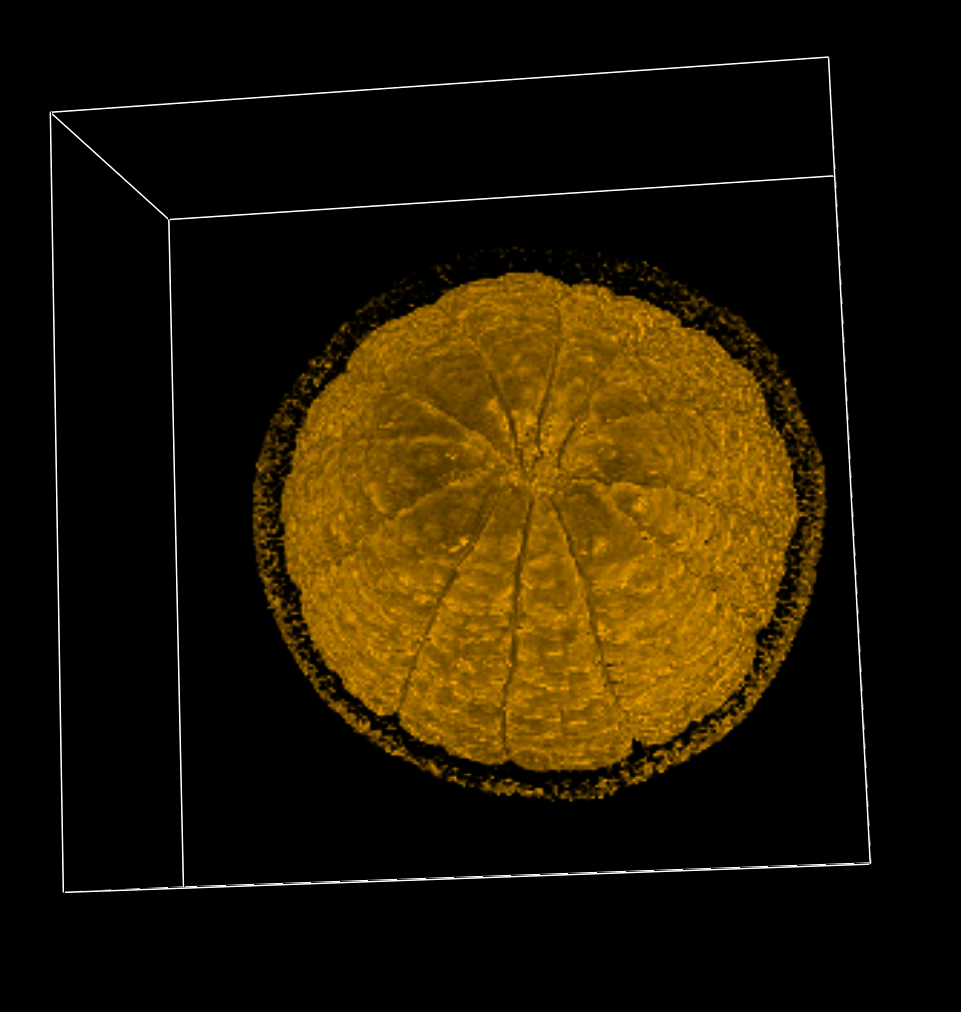
\includegraphics[width=\textwidth]{trilinear-off}
    \caption{Trilinear interpolation disabled.}
  \end{subfigure}
  \hfill
  \begin{subfigure}[b]{0.45\textwidth}
    \centering
    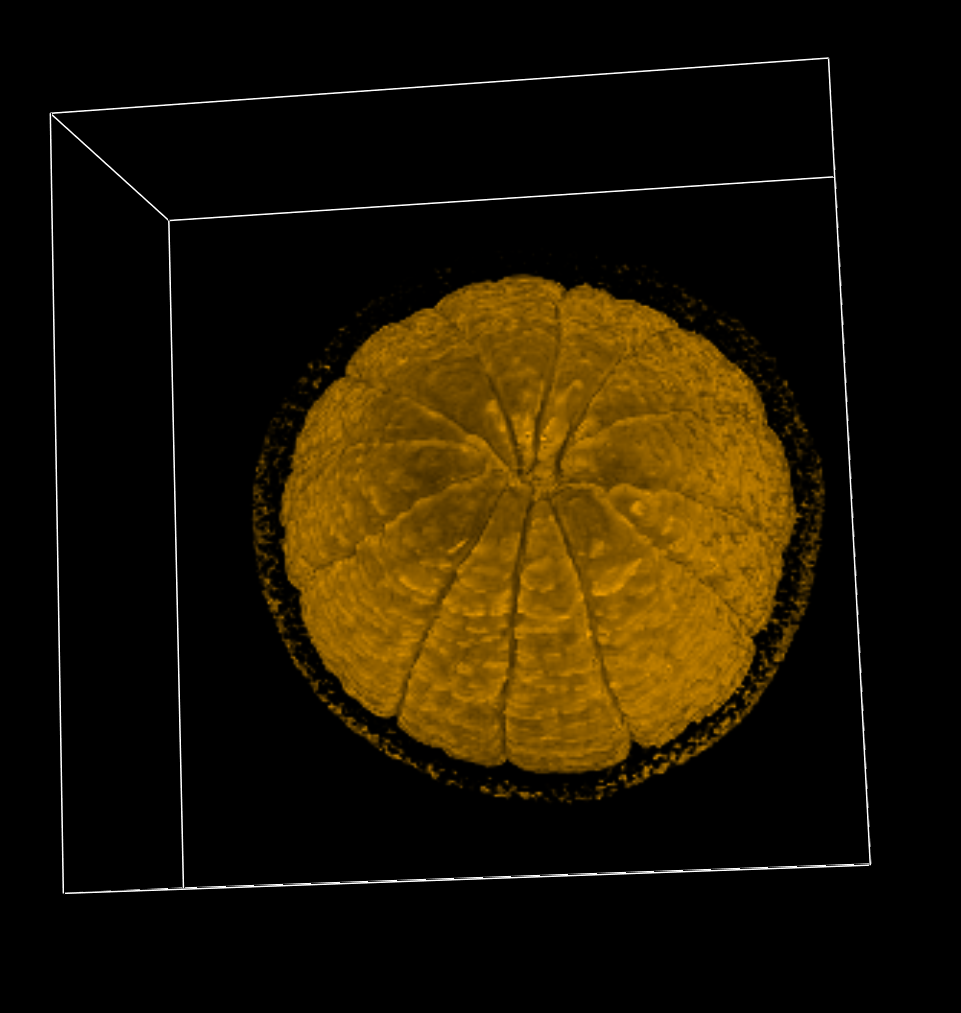
\includegraphics[width=\textwidth]{trilinear-on}
    \caption{Trilinear interpolation enabled.}
  \end{subfigure}
  \caption{Result of compositing visualization with and without trilinear interpolation on the \textit{orange} dataset.}
  \label{fig:trilinear}
\end{figure}

\begin{figure}[h]
  \centering
  \begin{subfigure}[b]{0.45\textwidth}
    \centering
    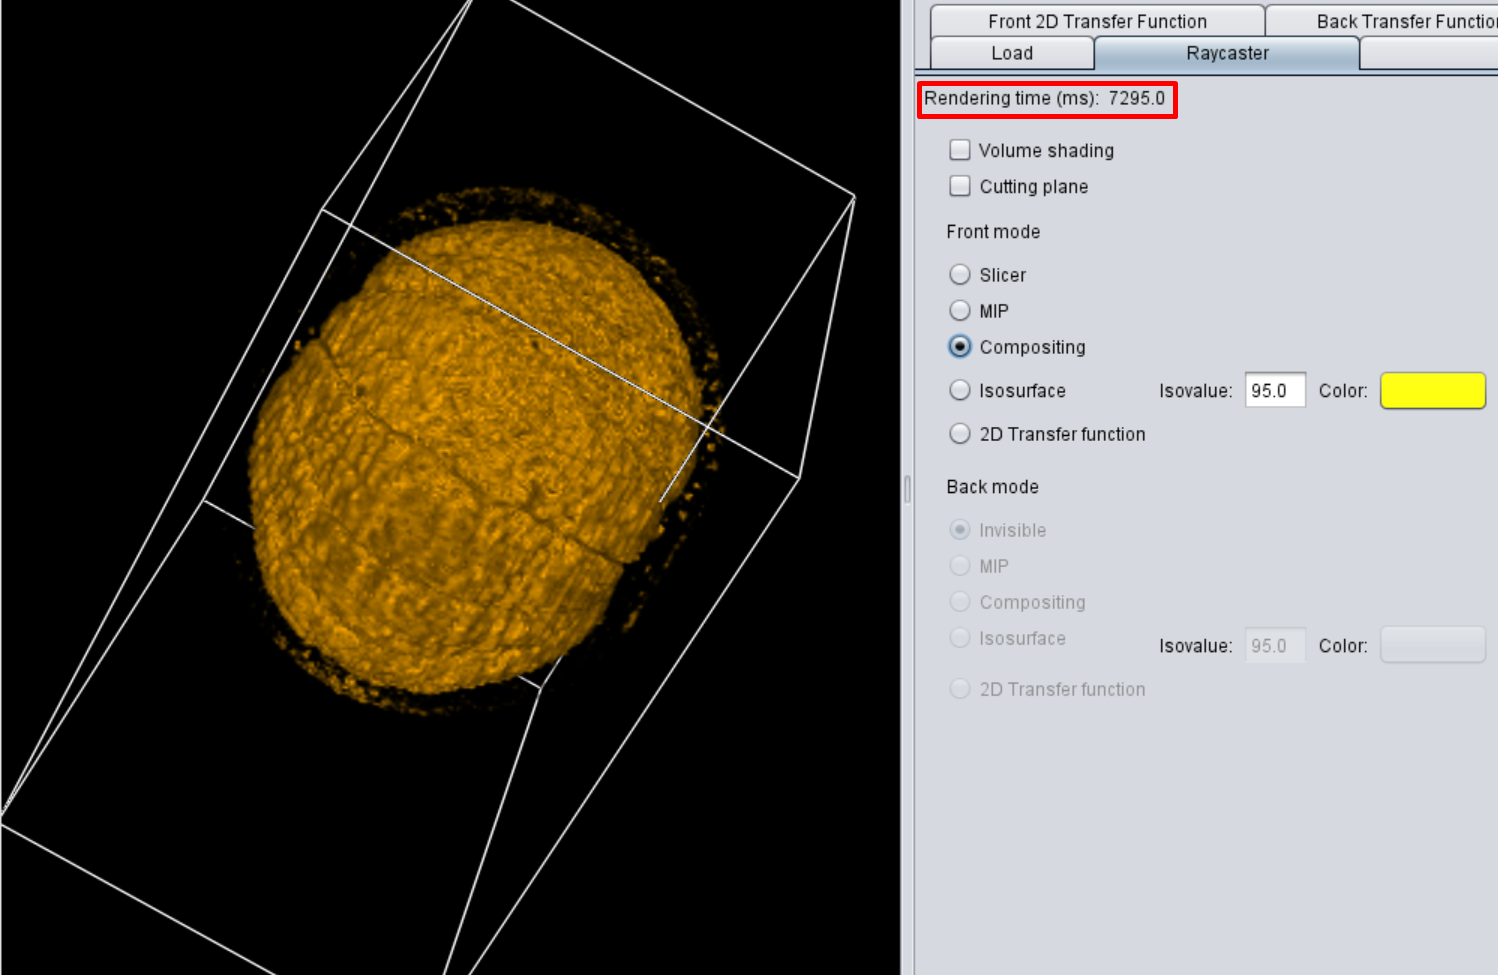
\includegraphics[width=\textwidth]{before-speedup}
    \caption{Interactive mode before speed up changes. Rendering time: 7295 ms }
  \end{subfigure}
  \hfill
  \begin{subfigure}[b]{0.45\textwidth}
    \centering
    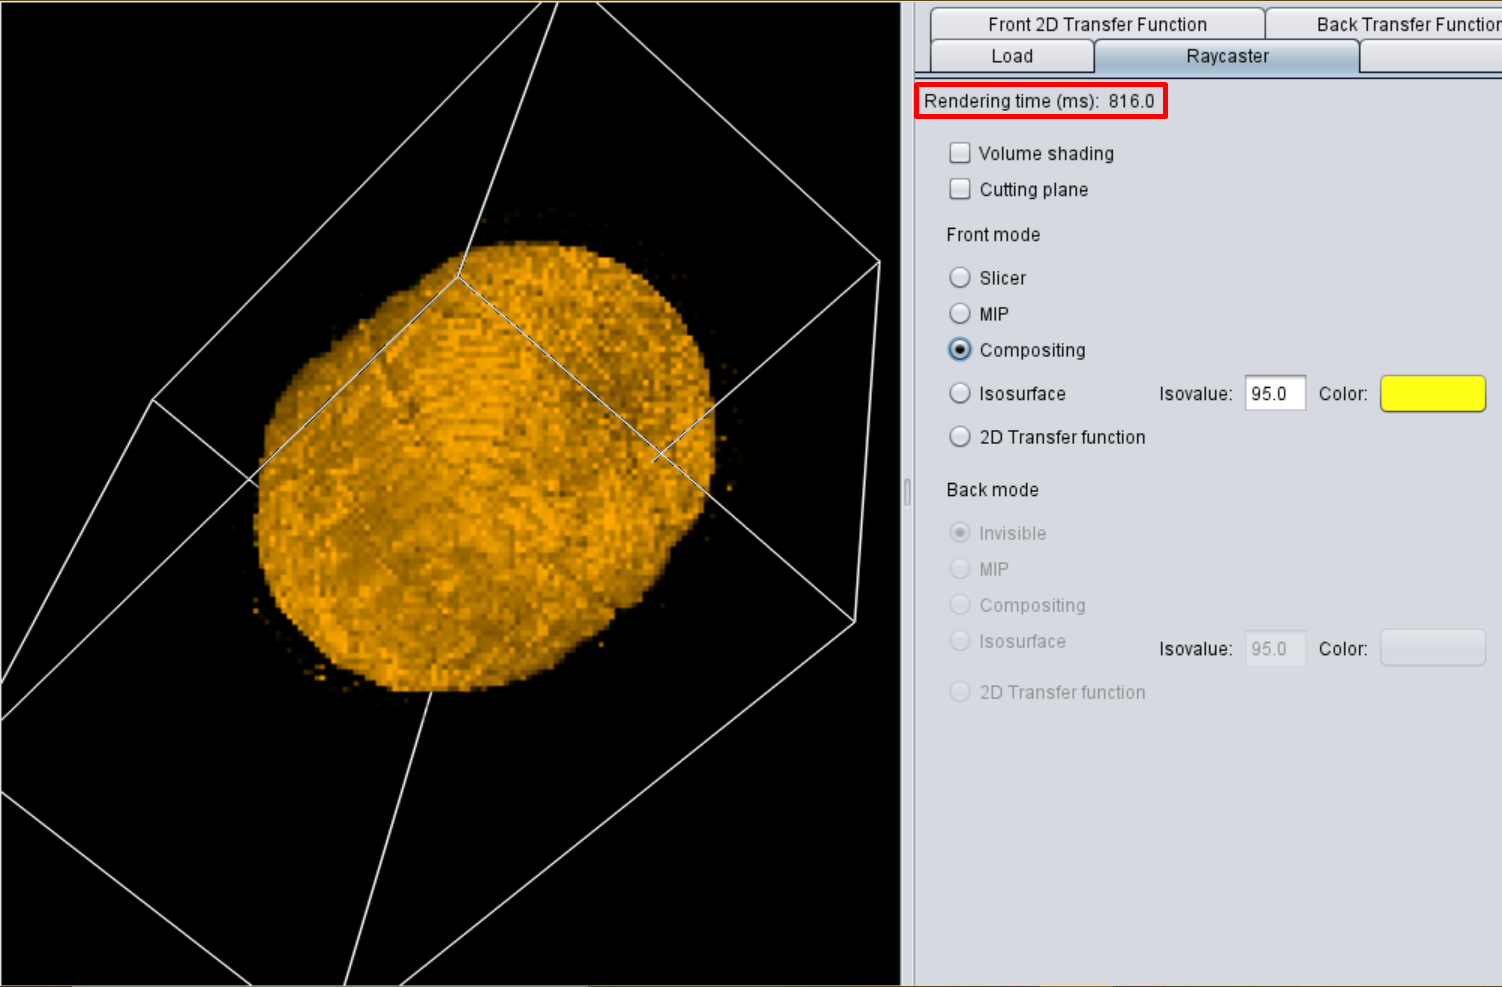
\includegraphics[width=\textwidth]{after-speedup}
    \caption{Interactive mode after speed up changes. Rendering time 816 ms}
  \end{subfigure}
  \caption{Result of speeding up interactive mode on the \textit{orange} dataset.}
  \label{fig:speedup}
\end{figure}

\begin{figure}[h]
  \centering
  \begin{subfigure}[b]{0.45\textwidth}
    \centering
    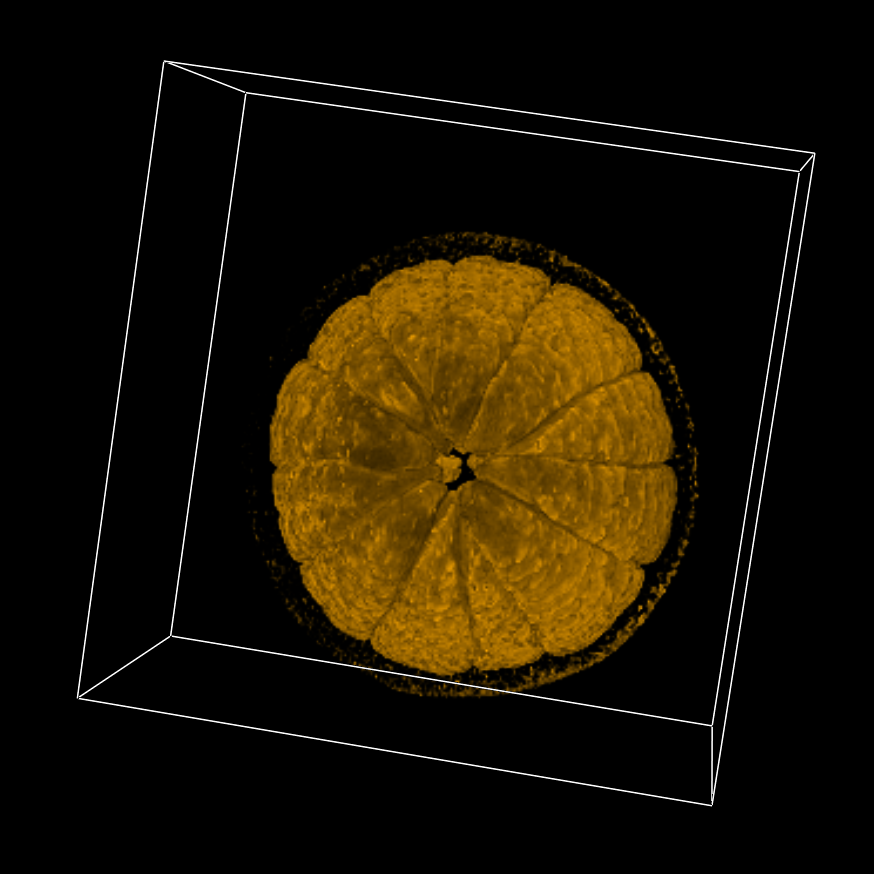
\includegraphics[width=\textwidth]{orange-composite}
    \caption{Composite with default values.}
  \end{subfigure}
  \hfill
  \begin{subfigure}[b]{0.45\textwidth}
    \centering
    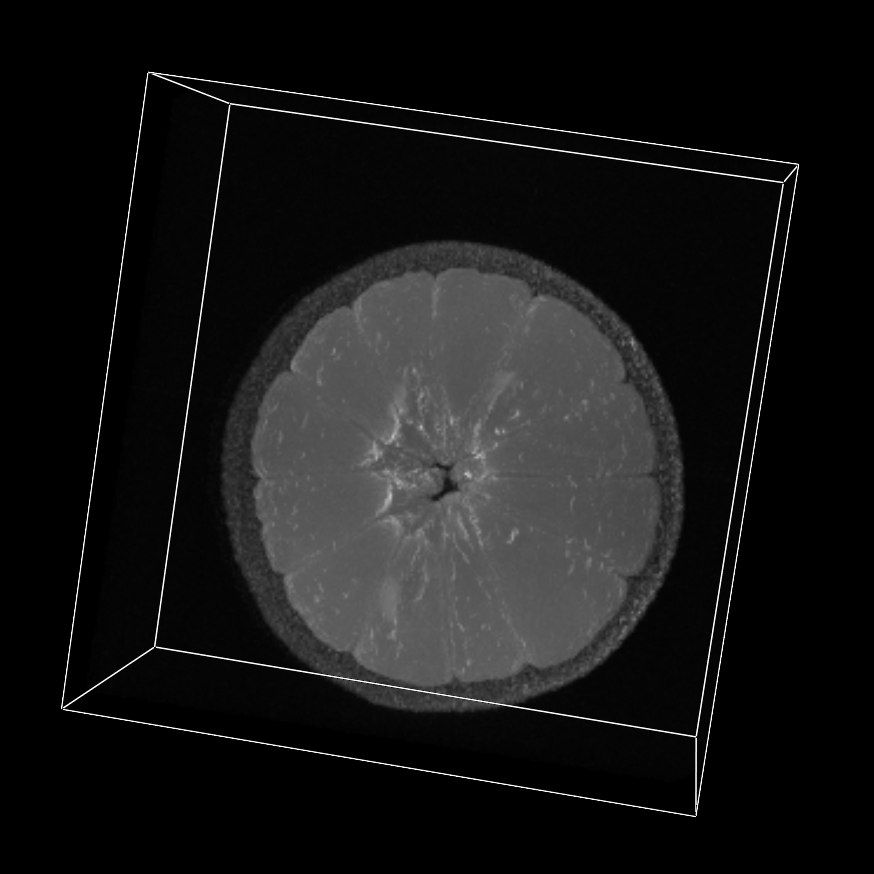
\includegraphics[width=\textwidth]{orange-mips}
    \caption{MIPS with default values.}
  \end{subfigure}
  \caption{Comparison of different raycasting techniques on \textit{orange} dataset.}
  \label{fig:mipscomp}
\end{figure}

\begin{figure}[h]
  \centering
  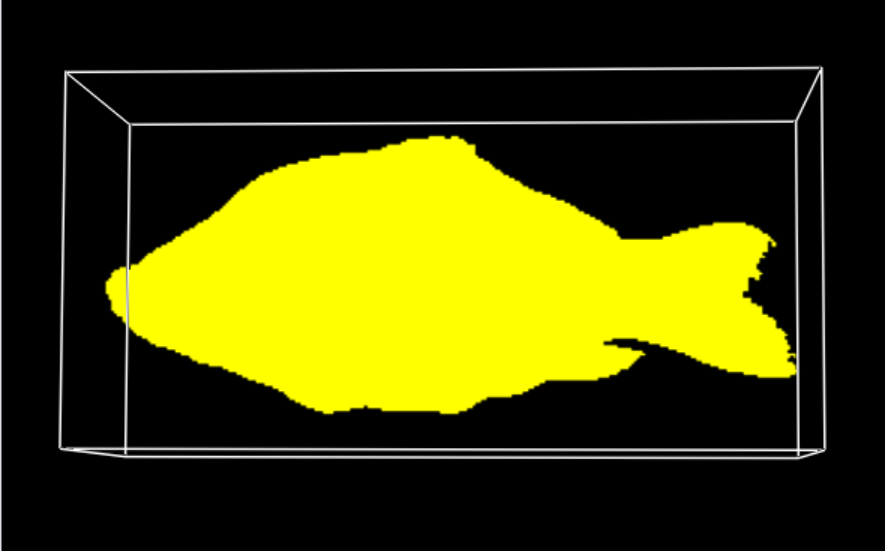
\includegraphics[width=\textwidth]{iso-surface}
  \caption{Isosurface raycasting without shading enabled on \textit{carp8} dataset.}
  \label{fig:isosurface}
\end{figure}


\end{document}
